\section{Introduction}
\setauthor{Romeo Bhuiyan}
\begin{figure}[htb]
  \centering
  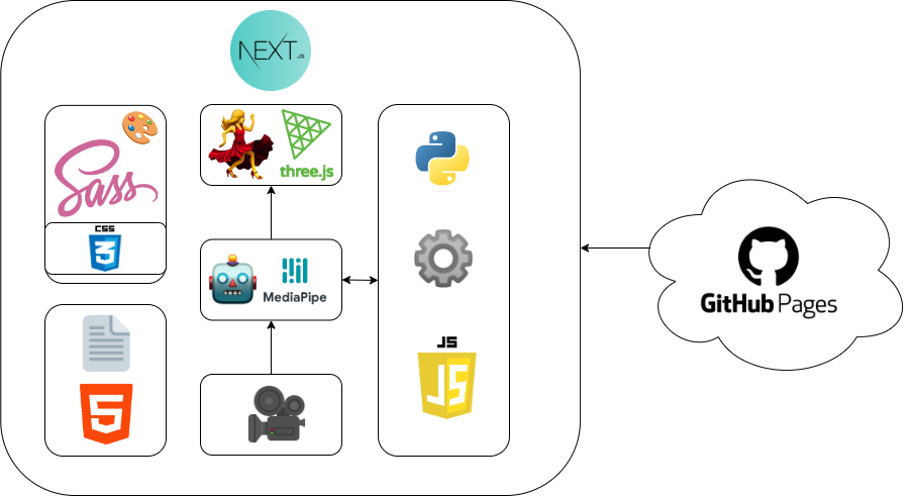
\includegraphics[width=0.9\textwidth]{pics/systemarchi.png}
  \caption{System architecture of Animotion}
  \label{fig:systemarchi}
\end{figure}

The figure \ref{fig:systemarchi} above shows the system architecture of Animotion which is 
designed to enable accurate and immersive face and body tracking experiences. 
The architecture incorporates various components and technologies to achieve seamless 
integration and efficient processing of movement data.

At the core of the system, the gestures and facial expressions are captured by a camera, typically a webcam. 
This visual data serves as the input for the tracking process. The captured data is then fed into the Mediapipe AI, 
as well as other script algorithms, for further analysis and processing. The movement data undergoes filtering 
processes within the script algorithms to extract the relevant information that will be utilized for tracking. 
This filtering helps to refine the data, ensuring that only the necessary movement data is used for subsequent stages.
Next, the processed movement data is applied to the Virtual Reality Model model, which represents the 
virtual character or avatar. This integration is achieved through the utilization of Three.js, a powerful 
web-based 3D graphics library, and the Three VRM.js library, which specializes in rendering VRM models. 
These technologies enable the visualization of the tracked movements on a canvas, providing users 
with a real-time representation of their gestures and mimics.

To support the web application framework, Animotion has chosen Next.js. 
This framework offers robust features for building web applications and facilitates seamless server-side 
rendering and routing. Additionally, the design aspect of Animotion's application is accomplished using Sass, 
a popular CSS preprocessor that enhances the efficiency and organization of styling code.
In terms of data loading, Animotion has implemented a locally loaded approach. The data, after being 
pulled from the web server, is stored and accessed locally. This approach ensures that users can run the 
application efficiently without relying heavily on continuous server connectivity. Animotion has employed 
GitHub Pages as the web server, leveraging its capabilities for hosting and serving the application content.

\section{Interactive 3D graphics with Three.js}
\setauthor{Romeo Bhuiyan}
Animotion encountered an initial hurdle in seamlessly integrating the VRM model onto the canvas 
and achieving smooth rendering. The objective was to accurately represent the tracked facial and 
body movements in real-time. This posed a significant challenge due to the complex nature of the VRM 
model and the requirement for seamless integration. To overcome this obstacle, Animotion turned to the 
powerful combination of Three.js and Three VRM.js libraries.

Three.js, a widely used web-based 3D graphics library, emerged as the foundation for 
Animotion's project. It offers an extensive range of tools and features, making it an ideal 
choice for creating interactive 3D applications within a browser environment. With its capabilities 
in rendering, animation, geometry manipulation, and material management, Three.js proved to be 
versatile and well-documented, supported by an active community.
For Animotion, Three.js played a crucial role in seamlessly integrating the VRM model onto 
the canvas. It provided a robust framework for rendering the 3D model, managing the scene graph, 
and handling user interactions. Animotion leveraged the capabilities of Three.js to manipulate and 
animate the VRM model based on the tracked facial and body movements, resulting in an immersive and interactive user experience. \cite{threejs}

\begin{lstlisting}[language=Python,caption=Loading the VRM onto the canvas,label=lst:vrmloading]
// VRM Loader
const loader = new THREE.GLTFLoader();
loader.crossOrigin = "anonymous";
// importing model from glitch.io our repo for storing the models
loader.load(
  window.localStorage.getItem("vrm"),
  (gltf) => {
    THREE.VRMUtils.removeUnnecessaryJoints(gltf.scene);

    // set the model infornt of user
    THREE.VRM.from(gltf).then((vrm) => {
      scene.add(vrm.scene);
      currentVrm = vrm;
      currentVrm.scene.rotation.y = Math.PI;
    });
  },

  (progress) =>
    console.log(
      "Loading model...",
      100.0 * (progress.loaded / progress.total),
      "%"
    ),

  (error) => console.error(error)
);
\end{lstlisting}


The provided listing above \ref{lst:vrmloading} showcases the implementation of loading and rendering a VRM using the Three.js library. 
The code addresses the challenges involved in seamlessly integrating the VRM model onto the canvas and accurately rendering it in real-time.
The first step is the initialization of the \texttt{THREE.GLTFLoader}, a loader specifically designed for handling models in the GLTF format. 
By setting the \texttt{crossOrigin} property to \emph{anonymous,} potential cross-origin issues when loading the VRM model are addressed.
Once the loader is set up, the \texttt{loader.load()} function is called to load the VRM model. During the loading process, 
a progress callback function is utilized to track the progress as a percentage. This provides feedback on how much of the model has been loaded.
Upon completion of the model loading, the success callback function is triggered. Within this function, 
the loaded model data is represented as a \texttt{gltf} object. However, before rendering the model, the unnecessary 
joints are removed using \texttt{THREE.VRMUtils.removeUnnecessaryJoints()}. This step optimizes the 
rendering process by eliminating any unnecessary components.
The \texttt{THREE.VRM.from(gltf)} function is then employed to convert the \texttt{gltf} object into a \texttt{VRM} object, 
suitable for rendering within the Three.js environment. The \texttt{VRM} object is added to the scene using 
the \texttt{scene.add(vrm.scene)} method, ensuring its integration into the overall scene graph.
To enable further manipulation, the loaded VRM object is assigned to the \texttt{currentVrm} variable. 
In the provided code, the rotation of the model is adjusted by setting \texttt{currentVrm.scene.rotation.y} to 
\texttt{Math.PI}, resulting in a 180-degree rotation around the y-axis.

Throughout the loading process, error handling is implemented with the error callback function. Any encountered errors 
are logged to the console, providing insight into potential issues that may arise.

While other libraries may offer similar functionalities, Animotion recognized that 
Three.js stood out as the preferred choice due to its versatility, robust features, 
and compatibility with the VRM model format. The combination of Three.js and Three VRM.js 
empowered Animotion to realize their vision and deliver a compelling face and body 
tracking experience that exceeded expectations.

\subsection{Rendering and manipulating VRM}
\setauthor{Romeo Bhuiyan}
Three VRM.js is an extension of the Three.js library specifically designed for working with VRM files. 
It provides a comprehensive set of tools and functionalities that enable developers to load, control, 
and render VRM models in real-time web applications. At its core, Three VRM.js leverages the capabilities 
of Three.js, a powerful web-based 3D graphics library. Three.js provides a solid foundation for creating 
interactive 3D applications, offering a wide range of features such as rendering, animation, and scene management. 
By building upon Three.js, Three VRM.js enhances its capabilities to handle VRM-specific functionalities and nuances.

The main functionality of Three VRM.js lies in its ability to load and parse VRM files. 
VRM files are industry-standard 3D model formats that contain information about the geometry, 
textures, bones, and blend shapes of a character, as shown in the figure below \ref{fig:threevrmdebug}. Three VRM.js streamlines the process of loading 
these files into a Three.js scene, automatically interpreting and organizing the data within the VRM file.
Once a VRM model is loaded, Three VRM.js enables developers to manipulate and control the model's 
behavior in real-time. It provides a variety of tools to handle complex tasks such as facial expression 
control, bone animation, and blend shape manipulation. Developers can dynamically adjust the model's 
appearance and behavior based on external input, such as tracking data from facial recognition or body tracking systems.
Another important feature of Three VRM.js is its support for Inverse Kinematics. \cite{threevrm}

To enhance performance and efficiency, Three VRM.js employs various optimizations. 
It utilizes the Graphics Processing Unit for hardware-accelerated rendering, 
ensuring smooth and responsive animations. Additionally, Three VRM.js incorporates 
techniques like Level of Detail management, which dynamically adjusts the level of detail
based on the distance between the camera and the model. This optimization improves 
rendering efficiency, particularly for complex scenes with multiple VRM models. \cite{threevrmgpu}
\\
\begin{figure}[htb]
    \centering
    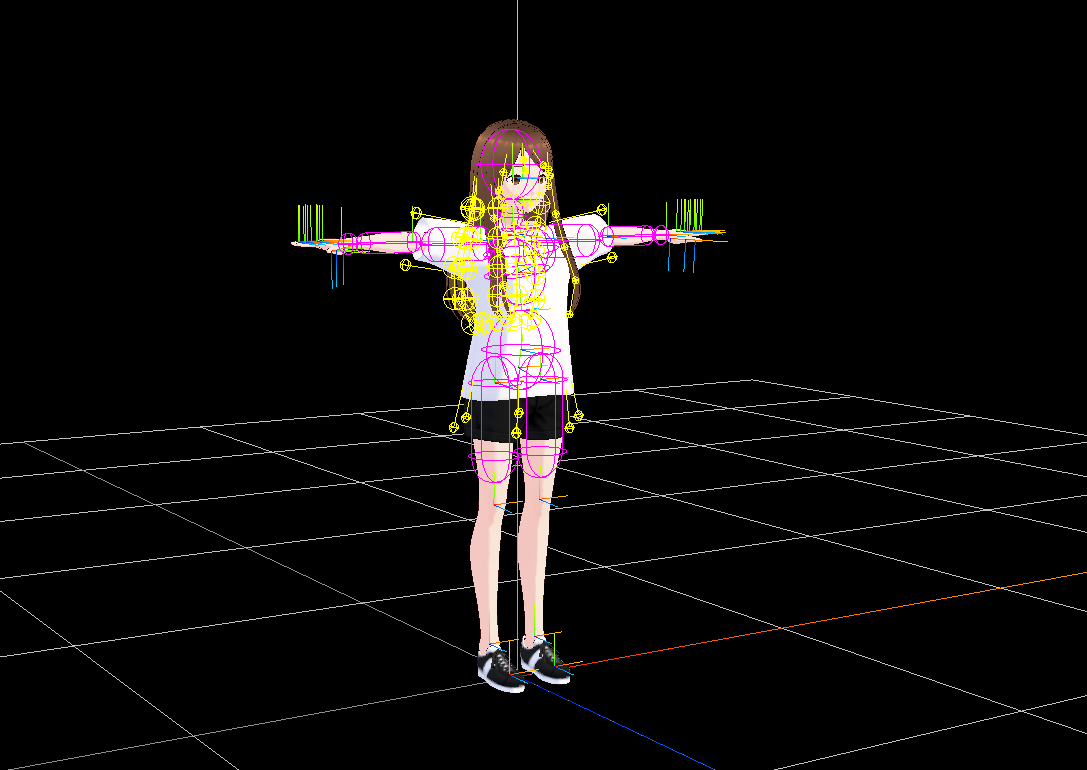
\includegraphics[width=0.9\textwidth]{pics/threevrmdebug.PNG}
    \caption{Three-vrm.js debug mode}
    \label{fig:threevrmdebug}
\end{figure}
\\

\subsection{Realistics movement with Inverse Kinematics}
\setauthor{Romeo Bhuiyan}
Inverse Kinematics (IK) is a technique used in computer graphics and animation to simulate realistic
 joint movement based on the desired position or orientation of an object's end effectors.
 In the context of Three VRM.js, which is an extension of Three.js for working with VRM models, 
 IK enables more natural and dynamic animations of the VRM models.
With IK, the position and rotation of the end effectors, such as hands or feet, are specified, and the IK 
solver algorithm calculates the appropriate joint angles required to achieve those positions. This allows for 
smoother and more realistic movements of the VRM model's limbs, making it appear as though the 
model is reacting to the user's input or the surrounding environment. \cite{whatisik}

By incorporating IK in Three VRM.js, Animotion or developers in general can create more realistic and fluid animations of VRM models. 
This enhances the overall visual quality and immersive experience of the virtual characters, as their movements 
closely resemble the natural motion of human limbs. The ability to accurately simulate IK in VRM models adds another 
layer of realism and expressiveness to the animations and interactions in applications by Three VRM.js. \cite{ikinthree}

\section{Decision between web frameworks}
\setauthor{Christoph Lasinger}
The decision to use a web framework at all and not simply vanilla HTML, CSS and JavaScript came from a multitude of reasons.
For example, all the ways they provide assistance while developing, such as providing a file structure in which to neatly 
organize a project, a prebuilt routing system, a template-project that can serve as starting point, an option to debug a 
project and many more. As a result, a great amount of both time and effort can be saved, that can then in turn be spent on 
those particular parts of the project that are actually important.

Another reason to use web frameworks that has less to do with development, but more with working as a software engineer in 
the real world, is that for a lot of jobs experience in working with certain frameworks is certainly very useful, if not 
even required. The following graph \ref{fig:WebframeworkJobs} shows a breakdown of about 650 000 job offerings on websites like Linkedin, 
Dice and Glassdoor by the required framework \cite{WebframeworkJobs}.
\\
\begin{figure}[htb]
  \centering
  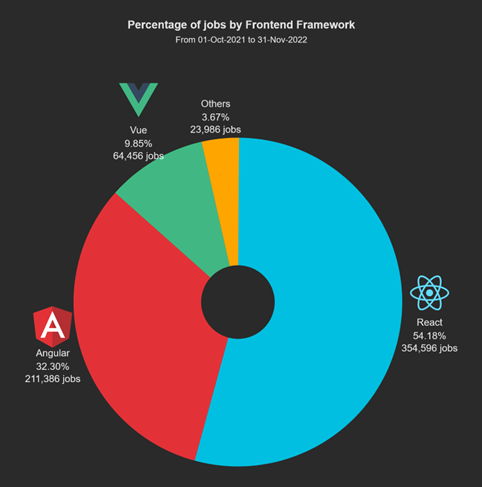
\includegraphics[width=0.7\textwidth]{pics/piechartwebframework.png}
  \caption{Breakdown of job offerings by framework}
  \label{fig:WebframeworkJobs}
\end{figure}
\\
\section{Angular}
\setauthor{Christoph Lasinger}
Angular, the next version of the discontinued AngularJS, is a framework for single-page applications (SPAs) and is maintained and released
by Google in 2016. An SPA is a type of web application that dynamically rewrites the current webpage instead of entirely reloading, i.e.,
requesting and displaying data from the server, it. The main benefits of SPAs are a more responsive user experience and avoiding the delay
of having to wait for a website to load. \cite{RoadToReact}
% is this really a good description of Angular?
\\
Angular is a free and open-source project, meaning that the copyright owner, in this case the company Google,
gives anyone the right to distribute, modify and study the software for any purpose. Open-source software is 
however not the same as public-domain software as it still possesses a copyright, just a very open one, hence its name. 
One big advantage of such software over closed-source software is that anyone in the world can find bugs and make 
improvements for it, free of charge for the actual project-owner. Moreover, even if the publisher decides to no longer 
provide support and update their software, it can still be adapted and improved by its users. Amazingly, it can be seen 
in practise that this concept works and users really do improve open-source projects not only for their benefit but for 
that of others as well. For those reasons, Animotion too is an open-source project \cite{Opensource}.
\\
Concretely, Angular is a web framework, built on Typescript, a high-level, object-oriented programming language that is 
a superset of JavaScript, that can be used to build from small projects to enterprise-grade web applications. It has a 
large library-collection that covers a wide array of features and offers an equally large number of developer tools for 
testing, updating and maintaining one's code. Moreover, Angular is component-based, meaning that an application consists 
of several building blocks (components), whereas each one defines one part of the user interface and any behaviour associated 
with it. Because these components are reusable and effectively modularize the application, it becomes easier to develop and 
test and makes the code more readable. This effect is especially noticeable in large-scale projects \cite{AngularDescription}.
\\
The Angular \gls{cli} plays a big part in development as it is used to efficiently and 
conveniently create, build, and test Angular applications by using the commands \texttt{ng new}, \texttt{ng build}
and \texttt{ng test} respectively. It can also be used to add new libraries through \texttt{ng add}
when needed. However, the most important command when developing is ng serve, as it starts the application on
localhost and automatically rebuilds it and reloads the website if any changes to the source code occur, which makes 
developing more convenient \cite{AngularCLI}.
\\
\section{React}
\setauthor{Christoph Lasinger}
Like Angular, React also is an open-source SPA-Framework, released by Meta (then Facebook) in 2013 and maintained by
Meta and a community of developers. Although the main focus of React lies on the component system and its DOM, it also 
has a large ecosystem of libraries surrounding it, making React flexible in terms of its uses.
% one more sentence?

\subsection{Virtual DOM}
\setauthor{Christoph Lasinger}
As mentioned before, among the most notable features of React is its virtual DOM (Document Object Model), a type of 
data structure that represents a webpage making it possible to only update certain parts of it that have changed. 
This provides a major performance boost but does not create extra effort for the developer as they can still write 
code as if the entire page is re-rendered on each refresh.

\subsection{Components}
\setauthor{Christoph Lasinger}
As React is a component-based framework, the feature of components is one of its main concepts. Concretely, they
allow the UI of a website to be split up into many reusable, independent parts,
for example a button, an input form, a dialog, and so on. In the programming language of React, JavaScript,
components can be either implemented through functions, so-called function components, or classes, which is done 
more commonly as they provide more features. In general, React components work like a function, they are handed 
arbitrary inputs which are called props in the terminology used by React
and return UI elements that are displayed on the website. When creating 
such a class the minimum requirements are that it extends the base component class React.Component, though it 
also possible to define one's own base class it is strongly discouraged in the official documentation of React,
and that it defines a method called render \cite{ReactComponentProps} \cite{ReactComponent}.
\\
\subsection{React JSX}
\setauthor{Christoph Lasinger}
React JSX is an abbreviation of JavaScript XML and a combination
of HTML and JavaScript. It plays a big part in React as JSX is the return type of all components. The following 
code snippet shown in listing \ref{lst:react} serves of an example.

\begin{lstlisting}[language=Python,caption=Example of a react component,label=lst:react]
  export default function About() {
  return (
    <>
    <button className="back-button" onClick={() => { GoTo("/"); }}>
      <p>back to menu</p>
    </button>
    <h1 id="main-headline" className="glitch" data-text="Community">Community</h1>
    <p className="community-text">
        Welcome to the community of Animotion! <br />
        Here you can join our official discord server and get to know new people. <br />
        You can also upload your own music and dance videos. <br />
        If you need help our 24/7 support is always here for you.
    </p>
    <iframe className="discord-iframe" src="https://discord.com/widget?id=1035647726634934382&theme=dark" allowtransparency="true" frameBorder="0" sandbox="allow-popups allow-popups-to-escape-sandbox allow-same-origin allow-scripts"></iframe>
    </>
  )
}
\end{lstlisting}

This exported function called About is, besides any imports that occur above it, practically the only code that makes 
up a so-called page, which exactly translate to a webpage, i.e., what comes up after visiting an URL. This function 
that shares its name with the file, a JavaScript file to be exact, merely consists of one long return statement that 
contains multiple HTML elements making up the webpage \cite{ReactJSX}.
The empty opening and closing tags at the beginning and end of the statement is the short syntax for a fragment, a 
feature in React that acts as a container and allows returning multiple child elements in a return statement 
without adding additional nodes to the DOM \cite{ReactFragments}.
\\
\subsection{Creating an Angular project}
\setauthor{Christoph Lasinger}
The easiest way to set up a React project is to use the officially supported command \emph{create-react-app}
(a similar command exists for Next.js, namely \emph{create next-app}) as it offers a modern build setup and is already preconfigured. 
Optionally, further parameters can be used to customize the project, for example \emph{—template typescript} to use TypeScript 
instead of JavaScript. After the project is created, it can immediately be started and viewed on localhost using either 
\emph{npm start} or \emph{yarn start}, depending on the package manager that is used. For development the command \emph{npm run dev} is 
also very useful, as the website is immediately refreshed after saving any changes to the code \cite{create-react}.
\\
\subsection{Comparison between Angular and React}
\setauthor{Christoph Lasinger}
In many regards React is similar to Angular, as they are both popular, component-based, open-source web frameworks. However, one 
significant difference that is especially important for beginners who have never worked with either one before lies in the 
steepness of their learning curves i.e., the one of Angular is much steeper than the one of React, meaning React is much easier 
to learn than Angular.

Additionally, in terms of popularity the gap between the two overall only seems to increase, with React coming out on top. This 
matters not only in the impact of demand on the job market but also in the size of the community. Because both projects are 
open-source a larger community means more active development, faster bug fixes, increased longevity, more chances of assistance 
in forums, and so on.

Another difference to consider when choosing one over the other is their respective programming language. While Angular is built
on TypeScript, React is a JavaScript library, so previous experience with one or the other, in case of TypeScript probably
more so the lack of experience, might influence the decision \cite{AngularReactComparison}.

While Animotion started out as an Angular project, after a short period of time we decided to use React instead, because it 
is easier to learn and more popular as well, as can be seen in figure \ref{fig:webpop} below. This graph shows the amount of 
searches for the npm packages of Angular represented in blue and React represented in orange in the past two years on
the npm trends website \cite{AngularReactPopularity}.
\\
\begin{figure}[htb]
  \centering
  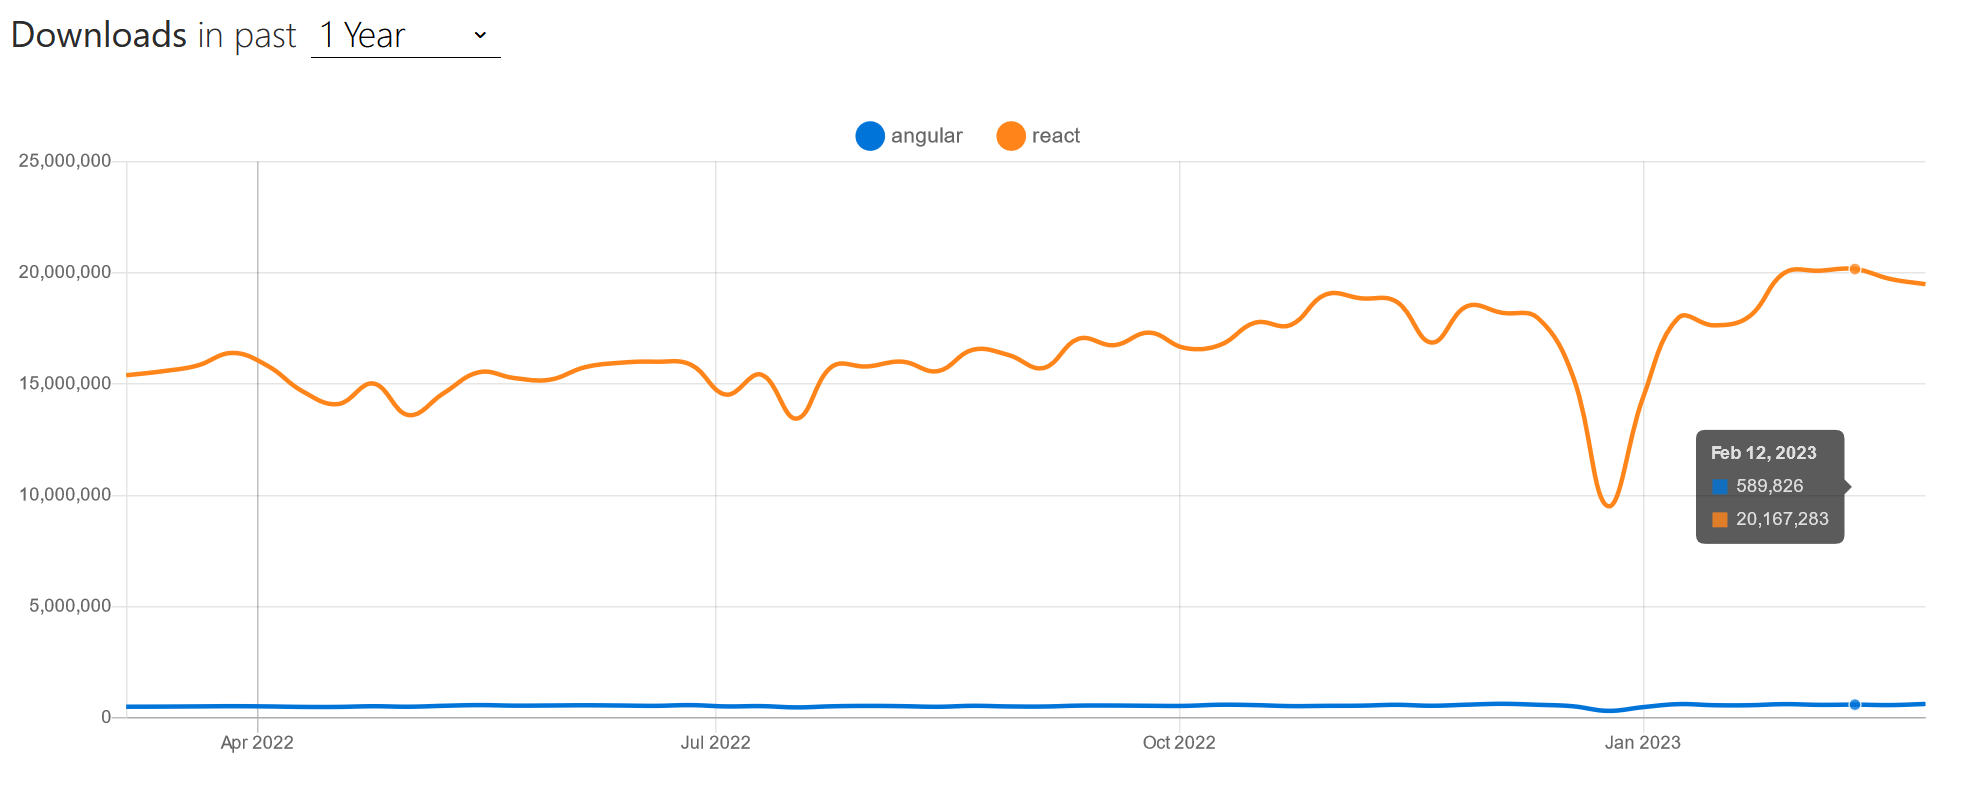
\includegraphics[width=1\textwidth]{pics/WebframeworkPopularity.png}
  \caption{Popularity of Web Frameworks}
  \label{fig:webpop}
\end{figure}
\\
Moreover, while we had some previous experience with JavaScript, we had never worked with TypeScript before, which made the attempt 
to understand Angular even more difficult than it needed to be. The comparatively better scalability of Angular was also not needed
for our project as it not likely to expand and therefore need for resources in the future.

\section{Next.js}
\setauthor{Christoph Lasinger}
Next.js is a React framework, meaning that, while React provides functions and features to build user interface elements
as a JavaScript library, Next.js handles the configuration and tooling that React needs. Additionally, Next.js provides
new features, structures, and optimizations. These additional features include data fetching, integrating, routing,
and so on \cite{NextjsDescription}.
\\
\subsection{Pages}
\setauthor{Christoph Lasinger}
One feature of Next.js that one will notice immediately is the representation of a webpage in JavaScript (or TypeScript) files as
so-called pages. In essence, they are React components that correlate to a route according to their file name (dynamic routing) and
have certain behaviours built into them from the moment of their creation.

For example, by default every page is pre-rendered, meaning that the HTML code of a webpage and as little JavaScript code as possible
that is required to perform its functions is generated in advance, instead of it having to be built from the JavaScript source code by
the client. This results in better performance and improves SEO, which means Search Engine Optimization and describes the process
of improving one's website in order to increase its visibility to search engines (e.g., Google).

In terms of implementing pre-rendering Next.js offers two general approaches: 
\begin{itemize}
  \item Static generation, which generates the HTML code for a webpage once when it is built and reuses it when responding to any request after that
  \item Server-side rendering, SSR for short and also referred to as dynamic rendering, which generates the HTML code anew each time a request is made
\end{itemize}

Next.js offers the option to use either one of these pre-rendering
techniques or both in combination, where most pages are statically generated, and others are rendered on the server. In its official
documentation Next.js recommends the usage of static generation over SSR because of its better overall performance. However, server-side
rendering might be necessary in some cases, for example when some data that is fetched from an API and displayed on the website needs
to be frequently updated \cite{NextjsPages}.
\\
\subsection{Data fetching}
\setauthor{Christoph Lasinger}
When developing a website, it is common to need to frequently fetch data from a remote source in order to update whatever is displayed
on the website. Because data fetching can play such an important role, Next.js offers several different ways to do it, that one can choose
from depending on the specific requirements and use cases of one's application. As server-side rendering and static-site generation have already
been thoroughly explained, the focus of this paragraph lies on the other two methods instead, though it should be noted that they are used by
exporting a function called \emph{getServerSideProps} or \emph{getStaticProps} respectively.

In contrast to server-side rendering, Next.js also offers the
option of client-side rendering or client-side data fetching, where data is generally fetched at runtime and at the component level. As a
result, the content of a page only changes whenever new data comes in. Though this can negatively affect performance and load time of one's
website, client-side rendering can be useful when SEO is not of importance, and pages need to be updated very frequently based on fetched data.
For implementing this strategy Next.js offers the React hook library SWR (stale-while-revalidate), a cache invalidation strategy
of HTTP. Next.js strongly encourages developers to use it in its documentation, as it handles focus tracking, caching, revalidation, etc. The
other method of data fetching is called ISR (Incremental Static Regeneration) and allows developers to statically generate pages on a
per-page basis, without the need of rebuilding the entire website. In order to use it, a revalidate prop is added to the \emph{getStaticProps} function \cite{NextjsDataFetching}.
\\
\subsection{Code splitting}
\setauthor{Christoph Lasinger}
Another feature of Next.js is called code splitting, which is the process of splitting the bundle of an application into multiple smaller parts
required by each entry point, an entry point usually being a page. This is done in order to be able to only load the code required to run the one
page that is being viewed at the time, reducing the initial load time of the website as a result. It is to note that any code shared between pages
is split into separate bundles in order to have everything available that is needed to load a page. Additionally, Next.js makes it possible to
pre-load the code of pages that users commonly navigate to next, further improving user experience \cite{NextjsCodeSplitting}.
\\
\subsection{Image optimization}
\setauthor{Christoph Lasinger}
When it comes to performance Next.js offers a special Image component that extends the default image HTML element and should be used instead of
it as it has several advantages. For one, because of its performance optimizations and improved Core Web Vitals, metrics provided by Google that
measure end-user page experience, using Image components improves SEO. These optimizations include automatically serving images in their correct
size, resizing them on-demand if it is needed, and in modern formats, providing visual stability i.e., preventing the layout from shifting unexpectedly
and potentially causing errors, only actually loading the image if it can be seen by the user, etc. The actual images can be either stored locally
or loaded remotely and if there is an image on page that is especially important, perhaps very big or noticeable if absent, it can be given priority
when being loaded \cite{NextjsImageOptimization}.
\\
\subsection{Conclusion}
\setauthor{Christoph Lasinger}
After starting out with Angular and then switching to React, we ultimately decided to use Next.js for a number of reasons. For example, the built-in
routing system, very easy setup through the create-next-app command, aforementioned features that increase performance, the simplicity of its
file structure, namely all pages being in one folder, and so forth. Especially the gentleness of its learning curve had a big influence on the decision.

\section{Sass}
\setauthor{Christoph Lasinger}
Sass stands for syntactically awesome style sheets and is a stylesheet language that compiles into CSS (Cascading Style Sheets). It extends CSS by a number
of features such as functions, variables, nested loops, mixins, etc. As a result, Sass enables stylesheets to be organized more easily and for design
to be shared within and across projects. There are two syntactic variants i.e., versions of Sass, the most commonly used one being the SCSS syntax, where the
filename ends in .scss. It is a superset of CSS, meaning that all CSS code is also valid SCSS code. The other version of Sass is called the Sass syntax
and is a bit more unusual i.e., sort of like the programming language Python it abandons the typical structure of curly braces and semicolons used in CSS
to separate and organize lines of code in favour of simple indents and newlines. However, apart from the different styling elements used, both syntaxes
are the same in all other aspects, including the features they provide. Since SCSS is a superset of CSS, one can simply write CSS code for the most part
and use any SCSS feature when it seems useful, which makes Sass very easy to learn and adopt \cite{SassFeatures}.
\\
\subsection{Variables}
\setauthor{Christoph Lasinger}
For example, instead of copying the hexadecimal value representing a colour for each and every element and possibly making mistakes, Sass makes it possible
to store the colour code in a variable and access it using its more human-readable name. This feature can be very useful when for example working with brand
colours or main themes, as in those cases it is important to consistently use the exact same colour each time \cite{SassFeatures}.
\\
\subsection{Inheritance}
\setauthor{Christoph Lasinger}
Another useful feature of Sass is inheritance, an example of which can be seen in the following code snippet \ref{lst:sass}.

\begin{lstlisting}[language=Python,caption=Textstyling in Sass,label=lst:sass]
  .default_text{
    text-align: center;
    color: white;
    font-family: Prototype;
  }

  .legal_notice_text{
    @extend .default_text;
    font-size: 0.5em;
  }
\end{lstlisting}

Through the \emph{extend} keyword CSS properties of one selector can be passed over to another selector which then automatically has the 
same properties set to the same values, thus inheriting them. In this example, legal-notice-text is merely a variant of the 
default-text and should therefore be of the same colour, font, and alignment. However, as legal-notice-text is of not much 
importance to the average user of the website, it should be rather small and take up little space. Because of the usage of 
inheritance, the code becomes more readable and easier to write and understand \cite{SassFeatures}.
\\
\subsection{Partials}
\setauthor{Christoph Lasinger}
When working on a very large project with a lot of different people file management and organization can certainly become difficult. In
these cases the partials feature of Sass can be of great use. It allows the separation of one big Sass file into multiple smaller ones,
thus modularizing it. These smaller files usually have names ending in \emph{(\_partials.scss}, where the underscore marks the file as one
that is not to be converted to a CSS file, and can be used in any other Sass files with the usage of the @use rule \cite{SassFeatures}.
\\
\subsection{Nesting}
\setauthor{Christoph Lasinger}
Other, smaller features of Sass include nesting, where multiple CSS selectors can be written under one, overarching selector creating a
clear visual hierarchy like in HTML, and the ability to use mathematical operators when for example calculating the width of a HTML
element, making the CSS more readable and the thought process behind certain values clearer, than simply using a specific number, like
575 pixels. There are also so-called mixins, basically reusable CSS selectors that can be customized in a specific instance by passing it
variables as parameters, that can be created using the @mixin rule and used with the @include rule \cite{SassFeatures}.
\\
\subsection{Conclusion}
\setauthor{Christoph Lasinger}
Overall, Sass has many useful features that in some cases can make a very big difference in terms of readability, level of organization and
convenience when writing CSS with no real downsides. Since Next.js has built-in support for Sass it is very simple to install and use right
away. For these reasons we decided to use Sass, specifically the SCSS syntax, for our project Animotion \cite{NextjsCSSSupport}.
\\
\section{Comparison of 3D rendering technologies}
\setauthor{Romeo Bhuiyan}
In order to display a virtual model on a canvas, a 3D rendering technology was required. Two libraries, 
GLTFLoader and WebGL, were evaluated using JavaScript to determine the best fit for the task at hand. 
The choice between the two ultimately depends on the specific needs and limitations of the project. 
Both GLTFLoader and WebGL are effective tools for rendering, but each have their own 
unique strengths and weaknesses.

\subsection{WebGL}
\setauthor{Romeo Bhuiyan}
WebGL is a powerful technology that would allow Animotion to harness the capabilities of hardware-accelerated 3D graphics within web browsers. 
It is an essential tool for creating interactive and visually stunning applications, including the face and body tracking 
functionalities that Animotion offers. WebGL stands for \emph{Web Graphics Library} and is based on the OpenGL 
ES standard, adapted to work with the web. \cite{WebGL}

One of the primary benefits of using WebGL for Animotion would be its ability to render complex 3D graphics directly 
within the browser without the need for plugins or additional software installations. This ensures broad 
compatibility and accessibility, as most modern web browsers support WebGL. Animotion could leverage this 
capability to deliver real-time 3D rendering of VRM models, enabling users to visualize and interact 
with their tracked facial and body movements seamlessly. Another advantage is WebGL's performance benefits are paramount. 
Utilizing the power of the Graphics Processing Unit, WebGL 
enables high-performance rendering and computation of 3D graphics, resulting in smooth and responsive visual 
experiences. This is especially crucial for face and body tracking applications where low latency and real-time 
responsiveness are vital to maintain a high level of user immersion and engagement. \cite{WebGLAdvantages}

Nevertheless, there are also some disadvantages associated with using WebGL. One notable concern is the potential for performance bottlenecks, 
especially on older or less powerful devices. While WebGL leverages hardware acceleration, it relies heavily on the Graphics Processing Unit, 
which can be a limiting factor on devices with weaker graphics capabilities. This could result in lower frame rates or reduced 
overall performance, affecting the smoothness of the face and body tracking experience. 
On top of that WebGL imposes certain security considerations. Since it provides access to the Graphics Processing Unit and hardware, 
malicious code executed through WebGL could potentially harm the user's system. Therefore, 
Animotion would need to implement proper security measures to prevent unauthorized access and protect users from potential threats. \cite{WebGLSecurity}

\subsection{GLTFLoader}
\setauthor{Romeo Bhuiyan}
GLTFLoader would be a valuable component for Animotion's face and body tracking system, enabling the seamless loading 
and rendering of 3D models in the GLTF format which stands for Graphics Library Transmission Format. GLTFLoader is a JavaScript library specifically designed to handle 
models in the GLTF format, which is optimized for efficient transmission 
and loading of 3D scenes and models. 
A big advantage of using GLTFLoader is the wide range of 3D models and scenes. 
GLTF is an open standard format that encompasses various types of 3D data, including geometries, materials, textures, 
animations, and more. This versatility would allow Animotion to integrate a diverse array of VRM models seamlessly 
into the face and body tracking system, ensuring a rich and immersive user experience.
Another advantage of GLTFLoader is its efficiency in loading and parsing 3D models. The GLTF format is designed 
for compactness and fast loading times, making it well-suited for web-based applications like Animotion. 
By using GLTFLoader, Animotion can minimize the loading times for VRM models, enhancing 
the overall performance of the face and body tracking system. \cite{GLTFLoader}

Furthermore, GLTFLoader's seamless integration with Three.js, the popular 3D library used by 
Animotion, streamlines the process of rendering 3D models. Three.js provides a powerful and user-friendly framework 
for creating 3D graphics within web browsers, and GLTFLoader's compatibility with Three.js ensures that Animotion 
can easily incorporate VRM models into the overall scene graph. GLTFLoader also supports animations and skeletal animations, allowing Animotion to animate the 
VRM models in real-time based on the tracked facial and body movements. This would enable Animotion to provide 
a dynamic and interactive user experience, where users can see their own movements reflected in the 3D models in real-time. \cite{GLTFLoaderWithVRM}

While GLTFLoader offers numerous benefits, it is essential to consider potential disadvantages as well. 
One potential challenge is the complexity of 3D models and scenes, which could lead to larger file sizes 
and longer loading times. However, GLTF's optimized format and efficient loading process help mitigate this issue to a large extent.

\subsection{Conclusion}
In conclusion, GLTFLoader emerges as the optimal solution for Animotion's 3D graphics needs, 
offering significant advantages over WebGL. By leveraging GLTFLoader, Animotion can efficiently 
handle the loading and parsing of GLTF files
eliminating the need for extensive custom code development. This streamlined approach saves valuable 
time and effort, allowing the team to focus on refining the face and body tracking system.
The results of using GLTFLoader are highly promising as shown in the figure \ref{fig:gltfloader} below. 
Animotion can now offer users an immersive and 
interactive experience where their tracked facial and body movements are mirrored in real-time by 3D models. 
The efficient loading and rendering of VRM models using GLTFLoader enhance the overall performance and 
responsiveness of the face and body tracking system, ensuring a smooth and engaging user experience.
Considering the specific requirements of Animotion's project, the combination of Three.js and Three VRM.js 
libraries with GLTFLoader proves to be the best choice. This combination enables Animotion to seamlessly 
load and display VRM models onto the canvas, accurately representing the tracked movements in real-time. 
By adopting GLTFLoader, Animotion ensures a more efficient and effective utilization of Three.js 
and Three VRM.js libraries, further elevating the quality of their face and body tracking system.
\\
\begin{figure}[htb]
    \centering
    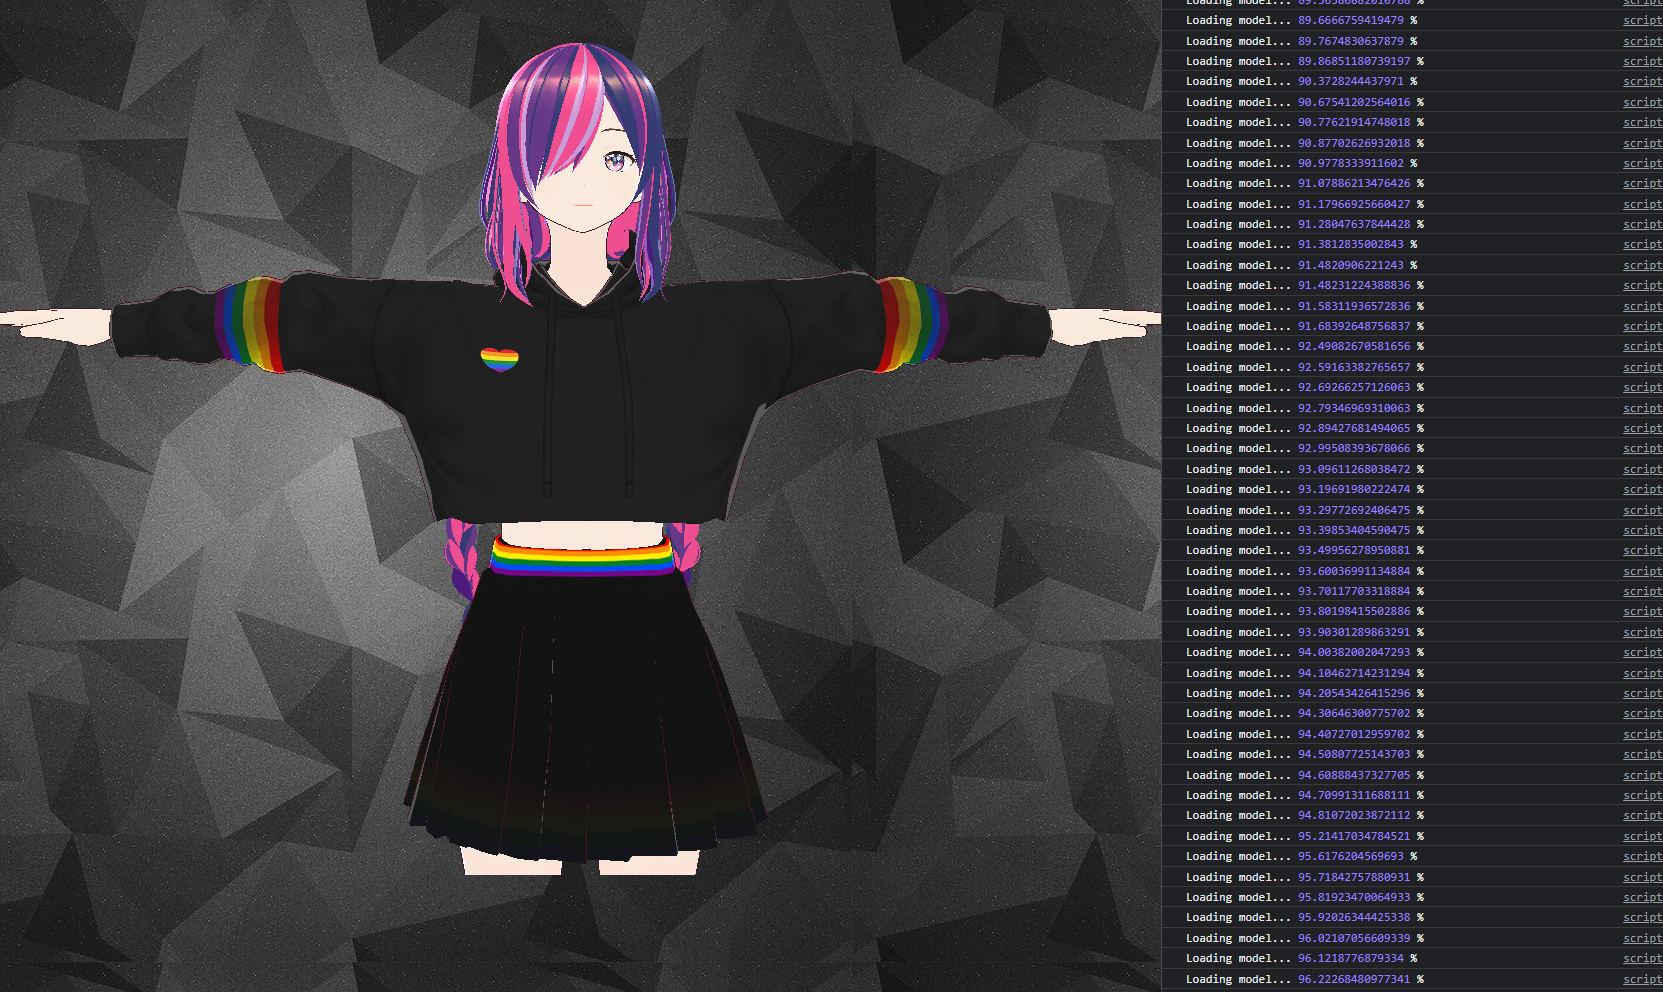
\includegraphics[width=0.9\textwidth]{pics/GLTFLoader.png}
    \caption{Loading the model with the help of GLTFLoader}
    \label{fig:gltfloader}
\end{figure}
\newpage
\section{Object interaction with OrbitControls}
\author{Romeo Bhuiyan}
Orbit-Controls.js is a JavaScript library used for controlling camera rotations 
and movements in 3D graphics applications. This library provides an easy-to-use 
interface for controlling the camera in a 3D environment, and is commonly used in 
interactive 3D web applications and other 3D visualizations.
OrbitControls.js is a critical component in Animotion's 3D graphics system, playing a important role in 
enabling intuitive camera control and user interaction. This library, built on top of Three.js, allows 
for smooth and effortless navigation of 3D scenes, offering users the ability to orbit around objects, zoom in and out, and pan the view.
In Animotion's context, OrbitControls.js is essential for providing users with a dynamic perspective of the tracked 3D models, 
enhancing their immersion and engagement. By incorporating OrbitControls.js, 
Animotion enables users to explore the virtual environment from different angles.

The usage of Azimuth and Polar angles in OrbitControls.js further enhances the control and customization options available to users.
The Azimuth angle, also known as the horizontal angle, allows users to rotate the camera horizontally around the tracked 3D 
model. On the other hand, the Polar angle, or vertical angle, empowers users to adjust the camera's position, 
providing flexibility in capturing different perspectives.
The combination of both angles in OrbitControls.js allows Animotion's users to view the 3D models from any desired viewpoint, 
which is especially crucial for face and body tracking applications. This feature enhances the possibilities of seeing the 
interactions from another point of view.

The most important advantage is that OrbitControls.js simplifies the implementation of camera control functionalities, 
reducing the development effort and ensuring a smoother user experience. By using the named libary, 
Animotion avoids the need to build complex camera control systems from scratch, saving valuable development time and resources.
\cite{orbitcontrols}

\subsection{Azimuth- and polar angle}
\setauthor{Romeo Bhuiyan}
The Azimuth angle and the Polar angle are two important concepts in 3D graphics and visualization. 
In the context of orbit-controls.js, they are used to control the camera's rotation and position in 3D space.

The Azimuth angle refers to the angle between a reference plane and the position of the camera in 
the x-z plane. This angle determines the camera's horizontal rotation and the direction it is facing. 
In orbit-controls.js, the Azimuth angle is controlled by moving the mouse horizontally.
The equation is given by: \ref{eqn:azimuth}
\begin{equation}
  \label{eqn:azimuth}
	azimuth = atan2(sin(\theta), cos(\theta)*sin(\phi) - tan(\phi)*cos(\theta))
\end{equation}
where theta represents the angle of inclination, measured from the horizontal, and phi represents the angle 
of rotation around the vertical axis, measured from the north.

The equation involves several trigonometric functions, including sin, cos, and tan, which describe the various 
components of the angle of inclination and rotation. The atan2 function is used to calculate the angle between 
the positive x-axis and the point (sin(theta), expression in parentheses) in the Cartesian plane.
The azimuth angle is an important parameter in many applications, including navigation, surveying, and satellite communications. 
It provides a convenient way to describe the direction of an object or location relative to true north, 
and can be used to determine the angle of elevation and other important parameters.
The Polar angle, on the other hand, refers to the angle between the position of the camera and the 
positive y-axis. It determines the camera's vertical rotation and the height of the camera relative 
to the scene. In orbit-controls.js, the Polar angle is controlled by moving the mouse vertically.
The polar angle, denoted by theta, is an angular coordinate system used in two-dimensional space to locate 
a point using a distance (r) and an angle (theta) measured from a fixed reference point.

It is the angle between the positive x-axis and the line segment 
joining the origin and the point (r, theta). The angle theta is measured in a counterclockwise direction 
from the positive x-axis, ranging from 0 to 2pi radians (or 0 to 360 degrees). The equation is: \ref{eqn:polar}
\begin{equation}
  \label{eqn:polar}
  \theta = arctan(y/x)
\end{equation}
where (x,y) are the Cartesian coordinates of a point in the plane. This equation finds the angle between the positive x-axis 
and the line segment connecting the origin and the point (x, y).
It is important to note that this formula works only when x is positive. If x is negative, 
then we must add or subtract pi radians (180 degrees) to the result, depending on the sign of y, to find the correct angle.
By controlling both the Azimuth and Polar angles, the orbit-controls.js library allows the user to 
change the position and orientation of the camera in 3D space. This is especially useful for interactive 
3D visualizations, where the user needs to be able to explore the scene from different perspectives, as shown below in the figure. \ref{fig:orbitcontrols}
Orbit-controls.js is often used in conjunction with WebGL and Three.js, which are libraries for creating 
3D graphics and animations in the browser. The combination of these technologies makes it possible to create 
interactive 3D visualizations that can run in a web browser, without the need for additional software or plugins.
\\
\begin{figure}[htb]
  \centering
  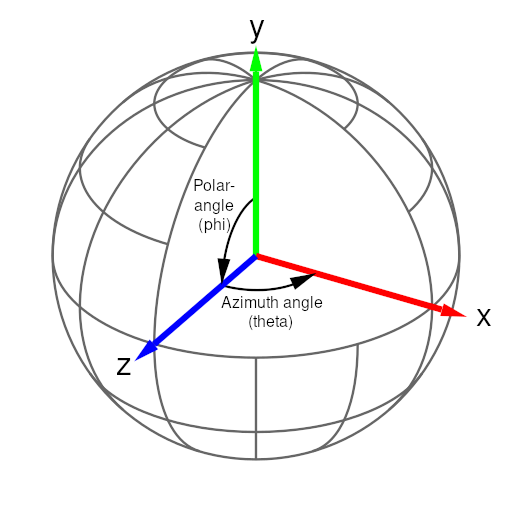
\includegraphics[width=0.5\textwidth]{pics/orbitcontrols.png}
  \caption{Azimuth and Polar angle}
  \cite{angles}
  \label{fig:orbitcontrols}
\end{figure}

\section{Camera utilization using Camera utils}
\setauthor{Romeo Bhuiyan}
Camera utils plays a vital role in Animotion's 3D graphics system, managing user input to effectively 
visualizing facial and body movements on the VRM model. As the backbone of camera control, Camera utils 
ensures a seamless and immersive experience for users to interact with the virtual environment.
This library plays a important role in capturing and representing the tracked movements on the VRM 
model in real-time. As users interact with the 3D environment, Camera utils records changing camera 
positions and angles, translating them into corresponding movements of the VRM model. This dynamic 
representation of the user's tracked facial expressions and body gestures fosters a highly 
interactive and engaging user experience. It simplifies the implementation of complex camera controls, 
saving valuable development time and resources for Animotion as shown in the pseudocode \ref{lst:camerautils} below. Its seamless integration into the 3D 
graphics system ensures a user-friendly experience, allowing users to focus on exploring and 
understanding their tracked movements without being hindered by technical complexities. \cite{camerautils}

\begin{lstlisting}[language=Python,caption=Camera utilization using CameraUtils,label=lst:camerautils]
  const camera = new Camera(videoElement, {
  onFrame: async () => {
    await sendVideoFrame(videoElement);
  },
  width: 640,
  height: 480,
  });
  camera.start();
\end{lstlisting}

The provided pseudocode \ref{lst:camerautils} above demonstrates the implementation of a camera module to capture video frames from 
a specified HTML video element \emph{videoEmlement} and process them using an asynchronous 
function called \texttt{sendVideoFrame}. The camera is set to capture video frames 
with dimensions of 640 pixels width and 480 pixels height. Upon starting the camera, it continuously captures 
and processes video frames in real-time, allowing developers to implement functionalities such as real-time video 
analysis, image recognition, or computer vision tasks. The \texttt{Camera} class provides a flexible and efficient 
solution for video frame capture and processing within web applications.

\section{Drawing movements with Drawing utils}
\setauthor{Romeo Bhuiyan}
Drawing utils are essential components of Animotion's user interface, using the real-time visualization of user 
input on the camera window. Their role is critical in displaying tracked facial expressions and body movements as 
they occur on the camera feed. By utilizing drawing utils, Animotion enhances the interactive nature of the 
application, providing users with intuitive feedback on their actions in real-time.
One of the primary reasons Animotion utilizes drawing utils is to overlay visual elements on top of the camera window to 
indicate the detected facial landmarks and body keypoints as shown in the listing \ref{lst:drawing} below. These visual cues serve as feedback to users, 
providing them with a clear understanding of how their movements are being tracked and interpreted by the AI system. 
For example, facial landmarks could be visualized as points on the user's face, while body keypoints could be 
represented as joints or markers, allowing users to see how their gestures and movements are being captured by the system.
Through the use of lines and shapes, Animotion provides users with valuable information and guidance during interactions. 
For example, drawing utils can help users maintain proper posture or movement alignment during exercises, ensuring precise execution. 
This interactive feature elevates the overall user experience and contributes to the effectiveness of 
Animotion as a valuable tool for tracking and analyzing movements. \cite{drawingutils}

\begin{lstlisting}[language=Python,caption=Setting the landmarks on the camera feed,label=lst:drawing]
  function drawResults(results):
    guideCanvas.width = videoElement.videoWidth
    guideCanvas.height = videoElement.videoHeight
    canvasCtx = guideCanvas.getContext("2d")
    canvasCtx.save()
    canvasCtx.clearRect(0, 0, guideCanvas.width, guideCanvas.height)
    drawConnectors(canvasCtx, results.poseLandmarks, POSE_CONNECTIONS, {color: "#a640ff", lineWidth: 4})
    drawLandmarks(canvasCtx, results.poseLandmarks, {color: "#f67d92", lineWidth: 2})
    drawConnectors(canvasCtx, results.faceLandmarks, FACEMESH_TESSELATION, {color: "#fcd4db", lineWidth: 1})
    if (results.faceLandmarks and results.faceLandmarks.length === 478):
        drawLandmarks(canvasCtx, [results.faceLandmarks[468], results.faceLandmarks[468 + 5]], {color: "#fcd4db", lineWidth: 2})
    drawConnectors(canvasCtx, results.leftHandLandmarks, HAND_CONNECTIONS, {color: "#FF1493", lineWidth: 5})
    drawLandmarks(canvasCtx, results.leftHandLandmarks, {color: "#a640ff", lineWidth: 2})
    drawConnectors(canvasCtx, results.rightHandLandmarks, HAND_CONNECTIONS, {color: "#a640ff", lineWidth: 5})
    drawLandmarks(canvasCtx, results.rightHandLandmarks, {color: "#f67d92", lineWidth: 2})
\end{lstlisting}

The pseudocode \ref{lst:drawing} shown above defines a function called \texttt{drawResults} that is responsible for visualizing the results of a tracking process on a canvas element 
named \texttt{guideCanvas}. The function takes \texttt{results} as an input parameter, which represents the tracked landmarks and connections from different body parts such as 
pose, face, left hand, and right hand. The first part of the function sets the width and height of the \texttt{guideCanvas} to 
match the video dimensions \emph{width and height} obtained from the \texttt{videoElement}.
The \texttt{canvasCtx} variable is created by obtaining the 2D rendering context from the \texttt{guideCanvas}, which allows drawing on the canvas.
Then, the \texttt{canvasCtx.save()} function is called to save the current drawing state before any changes are made.
The function clears the entire canvas by calling \texttt{canvasCtx.clearRect(0, 0, guideCanvas.width, guideCanvas.height)}, effectively removing any previous drawings.
Next, the function proceeds to draw the tracked landmarks and connections for the pose, face, left hand, and right hand using the \texttt{drawConnectors} 
and \texttt{drawLandmarks} functions with specific colors and line widths for each body part.

Drawing utils are essential for customizing the visual representation of tracked movements, 
making the interface more user-friendly and adaptable. Animotion can tailor the appearance of facial landmarks and body keypoints, 
choosing colors, shapes, and styles that align with the overall design and aesthetics of the application as shown in the figure below %. This customization allows Animotion 
to create a branded and consistent visual experience that resonates with its target audience.

\section{Screen capture technology}
\setauthor{Romeo Bhuiyan}
Screen capture technology can be really important in Animotion to record and showcase dance movements on their 
community site. This technology allows the capturing of visual content displayed on a computer screen, enabling Animotion to 
record dance performances and other interactions within their application or website. One of the biggest benefits is that Animotion can offer
its users the ability to record and share their dance performances effortlessly. 
By integrating screen capture capabilities into their platform, users can easily capture their dance routines, choreography, or creative 
movements directly from the application's interface. This empowers users to share their recorded dances on the community site, creating a 
sense of engagement and collaboration among the Animotion community. That technology also serves as a valuable tool for error 
detection and performance analysis. When users record their dance routines, they can review their movements and assess their 
performance with a critical eye. By observing the recorded video, dancers can identify areas for improvement, refine their 
techniques, and enhance their skills over time. This self-evaluation process can be invaluable in helping dancers to 
hone their craft and achieve higher levels of artistry. Screen capture can also help Animotion's team in finding potential 
performance errors or issues in the application. It enables developers and designers to record user interactions, including real-time 
tracking of facial expressions and body movements, which may not be immediately apparent through simple observation. By reviewing screen-captured 
content, the team can detect any discrepancies, glitches, or performance-related concerns that may go unnoticed by the human eye during regular testing.
There is also the benefit of sharing instructional content, tutorials, or demonstrations related to dance techniques or 
application functionalities. Animotion can create and distribute visual guides to assist users in understanding how to make the most of the 
platform's features and improve their dance recordings. This function can be viewed in the figure \ref{fig:examplevids} below. These instructional materials can elevate 
the educational aspect of the community site, encouraging a supportive learning environment and empowering users to explore and express their creativity freely.

\begin{figure}[htb]
  \centering
  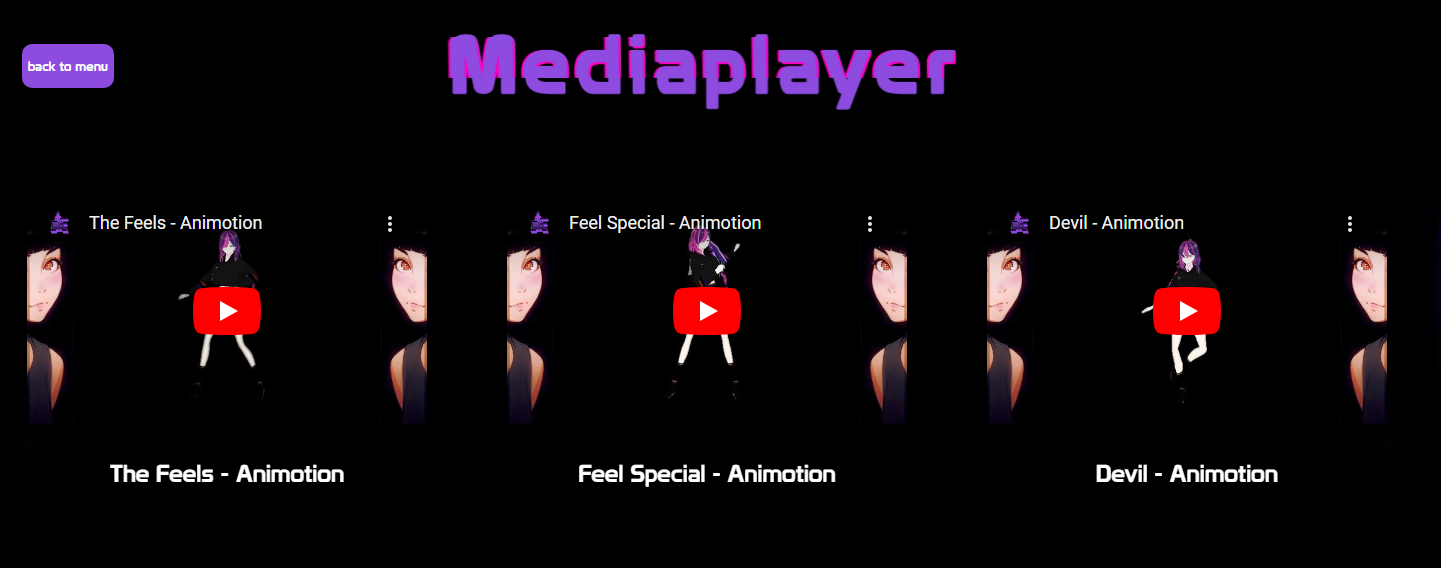
\includegraphics[width=0.5\textwidth]{pics/exampleVids.png}
  \caption{Instructional content provided by Animotion}
  \label{fig:examplevids}
\end{figure}

This discussed technology contributes to the documentation and archiving of dance performances. Through recorded videos, Animotion can preserve and 
catalog a diverse range of dance styles, genres, and expressions shared by the community. These recorded performances become an archive of artistic expression, 
having a sense of cultural preservation and promoting dance as an accessible and inclusive art form.

\subsection{RecordRTC}
\setauthor{Romeo Bhuiyan}
RecordRTC.js is a powerful and versatile JavaScript library that Animotion relies on for screen capturing capabilities within their platform.
This works by capturing the user's screen activity, including visual content displayed on the screen, audio input, 
and other media streams. The library utilizes the Web Real-Time Communication API, a modern web technology that enables real-time 
communication and media streaming between web browsers. Through this API, RecordRTC.js can access the user's multimedia devices, 
such as the microphone and camera, and capture audio and video data in real-time. \cite{rtcrecord}
When a user starts the screen capturing process on Animotion, RecordRTC.js starts capturing the specified media 
streams and converts them into a format suitable for recording and playback. The recorded content is then stored as a media file, 
such as a video or audio file, that can be saved or shared with others. This seamless recording process ensures that users can 
effortlessly document their dance performances and interactions within the application.
The library also offers various customization options, allowing Animotion to tailor the recording experience to its specific needs. 
For example, the library provides settings to control the quality, resolution, and frame rate of the recorded content, ensuring that 
users can capture high-quality dance performances. Additionally, Animotion can implement features like pausing, resuming, or 
stopping the recording to give users more control over the capture process. \cite{rtcrecord2}

\begin{lstlisting}[language=Python,caption=Starting the screen capture process,label=lst:recordrtc]
  function captureCallback(target):
    video.srcObject = target
    recorder = RecordRTC(target, {
        type: "video",
        mimeType: "video/webm",
    })
    recorder.startRecording()
    recorder.stopRecording(function):
        blob = recorder.getBlob()
        fileUrl = URL.createObjectURL(blob)
        video.srcObject = null
        video.src = fileUrl
        target.stop()
        recorder.save("screen_recording.webm")
        recorder.destroy()
        recorder = null
    end function
end function
\end{lstlisting}

The provided pseudocode \ref{lst:recordrtc} which can be viewed above outlines a function called \texttt{captureCallback}
that performs video capturing and recording tasks. When called, the function sets the media source of a video 
element to the specified media stream \texttt{target}. It then creates a recorder object using the RecordRTC library, 
configuring it to record video in the \emph{video/webm} format.
The function starts the recording process using the created recorder. Upon completing the recording, 
it executes the defined callback function. Within this callback, the recorded video is converted into a 
\emph{binary large object, also called blob} and transformed into a URL. The video element's source object is reset, and 
the recorded video is displayed by setting the video element's source to the created URL.
The function stops the media stream \texttt{target} to release the resources properly. 
The recorded video is saved as a \emph{screen\_recording.webm} file, and the recorder object is destroyed and set to null to free up memory.

\subsection{FFmpeg}
\setauthor{Romeo Bhuiyan}
FFmpeg.js and FFmpeg.min.js are powerful JavaScript libraries that bring the capabilities 
of FFmpeg, a renowned multimedia framework, to the web browser environment. These libraries seamlessly complement 
RecordRTC, another crucial component in Animotion's screen capturing system. RecordRTC is responsible for 
capturing video streams from user media devices, while FFmpeg.js and FFmpeg.min.js handle the post-processing tasks, 
such as video compression and format conversion. This combination creates a robust and comprehensive screen capturing 
solution that offers both real-time recording capabilities and advanced post-processing functionalities.
One of the key features that Animotion leverages is the ability to display conversion progress during video processing, 
as shown in the listing \ref{lst:ffmpeg} below. This progress indicator provides users with real-time feedback on the status of their video conversion.
By using these libraries, Animotion avoids the need for server-side processing, as all multimedia 
processing tasks are performed directly on the client-side. This approach contributes to a more efficient and 
responsive user experience, as there is no delay associated with uploading recorded videos to external servers for processing. \cite{ffmpeg}

\begin{lstlisting}[language=Python,caption=Showing the progress of conversion,label=lst:ffmpeg]
  ffmpeg = createFFmpeg({
    log: true,
    progress: showProgress,
  })

  function showProgress(ratio):
    if ratio is a valid number:
        Display the progress as a percentage
        message.innerHTML = "Complete: " + (ratio * 100.0).toFixed(2) + "%"
    else:
        Display an animated progress indicator
        if message.innerHTML is "/":
            message.innerHTML = "-"
        else if message.innerHTML is "-":
            message.innerHTML = "\\"
        else:
            message.innerHTML = "/"
\end{lstlisting}

The pseudocode \ref{lst:ffmpeg} showed above defines a function called \texttt{createFFmpeg()} 
to create an instance of the FFmpeg library with logging enabled and a progress callback function called \texttt{showProgress}.
The \texttt{showProgress} function handles the updates during video conversion. It displays the completion percentage if 
available or an animated progress indicator if the percentage is not yet available. This enables Animotion to show the 
conversion progress to users in real-time, enhancing the user experience.

\subsection{WebM video format for web-based applications}
\setauthor{Romeo Bhuiyan}
WebM is the ideal video format for Animotion due to its numerous benefits and compatibility with modern web technologies. 
WebM is an open and royalty-free video format developed by the WebM Project, which is sponsored by Google. It is specifically 
designed for web usage and is widely supported by popular web browsers, making it a perfect choice for Animotion's screen 
capturing and video sharing platform. It stands out as the preferred video format 
for Animotion due to its exceptional compression capabilities. Utilizing the VP8 or VP9 video codecs, WebM ensures 
efficient compression while preserving video quality at a high standard. This advantage is of paramount importance for Animotion, 
as it enables users to record and share videos with minimal file sizes, all while maintaining the integrity of visual details. 
The resulting reduction in file size not only leads to quicker video loading times but also facilitates smooth 
playback across the web, delivering an unparalleled user experience.
This video format also supports transparency through the VP8 alpha channel, allowing videos to have 
transparent backgrounds. This feature is highly beneficial for Animotion, as it enables the integration 
of screen-captured dance moves or gestures into various video editing software and platforms seamlessly. 
It also empowers users to overlay their captured content onto different backgrounds or compositions, 
enhancing the creative possibilities for their videos. \cite{webm}

\section{Calculation of the virtual reality model} 
\setauthor{Romeo Bhuiyan}
Controlling a VRM on a website involves a complex process that involves 
capturing the user's inputs, updating the VRMs position and orientation in real-time, 
and rendering the updated model for display on the user's device.
The first step in this process is for the user to interact with the VR model 
using a device such as a VR headset or a mouse and keyboard. The inputs from the 
user are then captured by the website and sent to the server. The server then 
uses these inputs to update the VR model's position and orientation in real-time. 

Once the VR model has been updated, it is then rendered, and the new frame is 
sent back to the user's device for display. This process repeats as the user 
continues to interact with the VR model. 
To achieve this, various technologies are needed such as GLTFLoader from the three
libraries for rendering the VR model in the browser, WebSockets for real-time 
communication between the client and server, and a physics engine to simulate 
the movement and interactions of the VR model. 

\subsection{Blendshape}
\setauthor{Romeo Bhuiyan}
Blendshape is an important technique that Animotion uses in its 3D animation and computer graphics to 
achieve seamless transitions between various shapes and expressions of a 3D model. This cutting-edge approach 
involves creating a collection of \emph{target} shapes for the 3D model, each representing distinct 
expressions or shapes. By utilizing a set of weight values or \emph{blend} values, Animotion can easily 
interpolate between these target shapes, resulting in fluid and natural transitions. The importance of this technique 
lies in enabling Animotion's AI to create a diverse array of expressive characters using a limited number of 3D models.

\subsection{Lerp}
\label{sec:lerp}
\setauthor{Romeo Bhuiyan}
The Lerp function, or Linear Interpolation, serves as a fundamental mathematical tool that Animotion 
utilizes to create smooth and seamless blends between two values. This function takes three essential 
inputs: a start value, an end value, and a weight. The weight acts as a vital factor, ranging from 0 to 1, 
signifying the precise proportion of the blend between the start and end values.
For example, if the weight is set to 0, the function will return the start 
value, and if the weight is set to 1, the function will return the end value. 
If the weight is set to 0.5, the function will return the midpoint between the 
start and end values. By adjusting the weight, the Lerp function can be used to 
smoothly transition between any two values over time.

Mathematically explained the linear interpolation, or simply interpolation, 
is a technique used to estimate values between two known data points. In other words, given two data points, 
interpolation allows us to estimate the value of a function at any point between those two data points.
The formula for linear interpolation is given by: \ref{eqn:lerp}
\begin{equation}
  \label{eqn:lerp}
	y = y1 + (x - x1) * (y2 - y1) / (x2 - x1)
\end{equation}
This formula is used to estimate a value between two known values on a straight line. It requires the following variables: y, 
which represents the estimated value; y1, the value of the dependent variable (y-axis) at the first known point (x1, y1); y2, 
the value of the dependent variable at the second known point (x2, y2); x, the value of the independent variable (x-axis) 
at which to estimate the value of y; x1, the value of the independent variable at the first known point; and x2, the value 
of the independent variable at the second known point.
The linear interpolation formula calculates the value of y by first determining the slope of the line connecting the two 
known points (y1, x1) and (y2, x2), and then extrapolating from that slope to estimate the value of y at the point x. 
This method is commonly used in scientific research when estimating the value of a variable at a point where it has not 
been directly measured, but falls within a range of values for which measurements have been made.

\begin{figure}[htb]
  \centering
  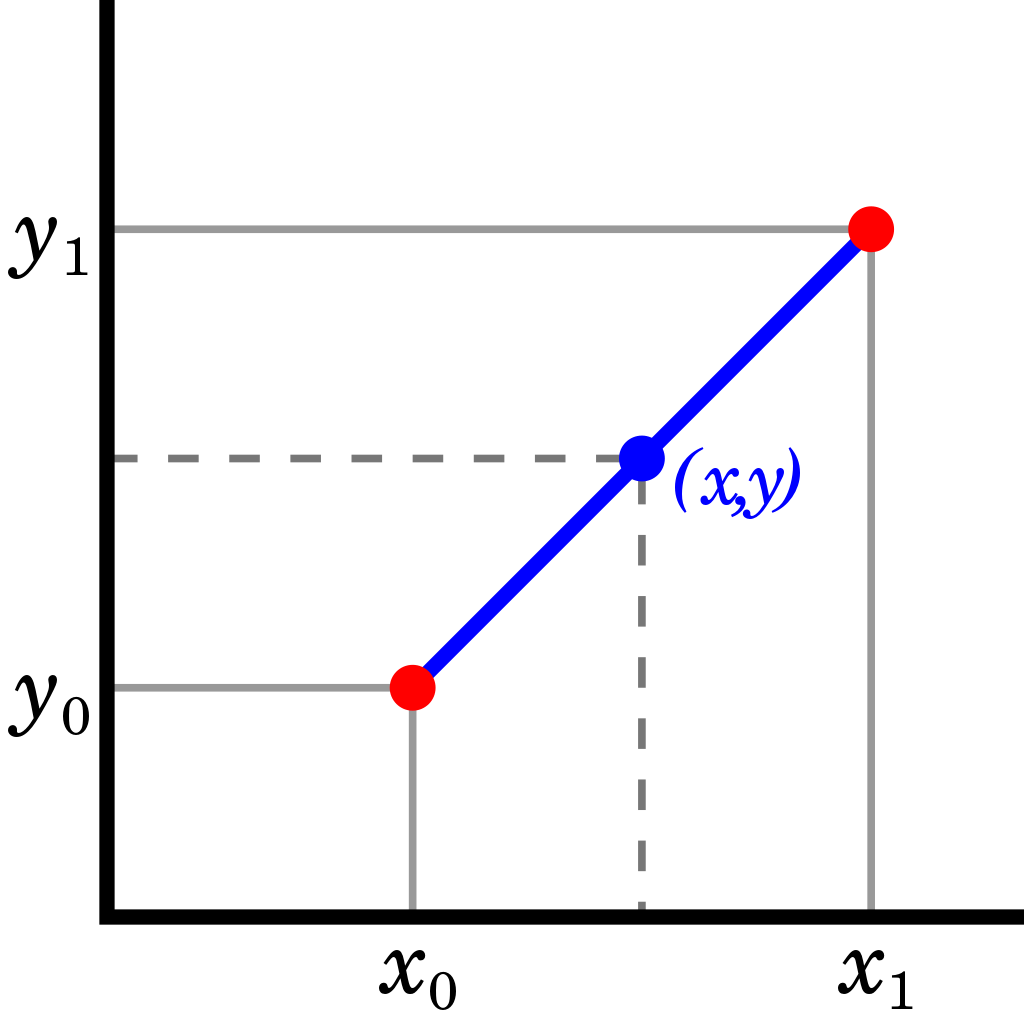
\includegraphics[width=0.4\textwidth]{pics/lerp.png}
  \caption{The blue line connecting the two red points is referred to as the linear interpolant, and it is used to estimate the value of y at a given x using linear interpolation.}
  \cite{angles}
  \label{fig:lerp}
\end{figure}

\subsection{Determining mouth expressions}
\setauthor{Romeo Bhuiyan}

\begin{lstlisting}[language=Python,caption=Shape of mouth,label=lst:shapeOfMouth]
    for each shape in ["I", "A", "E", "O", "U"]
        Blendshape.setValue(PresetName[shape], 
        lerp(riggedFace.mouth.shape[shape], 
        Blendshape.getValue(PresetName[shape]), 0.5))

\end{lstlisting}
As shown in the listing \ref{lst:shapeOfMouth}, this pseudocode is a loop that iterates over an array containing the shapes \texttt{A, E, I, O, U}. 
The purpose of the loop is to blend the shape of a rigged face's mouth with a preset value of a 
Blendshape object for each of these shapes. The loop starts by setting the value of the Blendshape 
object to a blended value between the shape of the rigged face's mouth \texttt{(riggedFace.mouth.shape[shape])}
and the current value of the Blendshape object \texttt{(Blendshape.getValue(PresetName[shape]))}. 
The blend is done using the lerp function, mentioned in above \ref{sec:lerp}. 
Quickly summarized, this function takes three arguments: the start value, the end value, and the weight of blending. 
In this case, the weight is set to 0.5, resulting in an even blend between the two values.
Once the blended value is calculated, it is set to the Blendshape object using the PresetName 
as the key. This process is repeated for each shape in the array, allowing the developer to 
easily blend the shape of the rigged face's mouth with preset values for multiple shapes.

\subsection{Blinking eyes}
\setauthor{Romeo Bhuiyan}
\begin{lstlisting}[language=Python,caption=Blinking of the eyes,label=lst:blinking]
    riggedFace.eye.l = lerp(clamp(1 - riggedFace.eye.l, 0, 1), Blendshape.getValue(PresetName.Blink), 0.5)
    riggedFace.eye.r = lerp(clamp(1 - riggedFace.eye.r, 0, 1), Blendshape.getValue(PresetName.Blink), 0.5)
    riggedFace.eye = Kalidokit.Face.stabilizeBlink(riggedFace.eye, riggedFace.head.y)
    Blendshape.setValue(PresetName.Blink, riggedFace.eye.l)

\end{lstlisting}
The pseudocode \ref{lst:blinking} shown above is a code block that performs blinking animation on a VRM model. 
The code uses the Lerp function, the clamp function, and the stabilizeBlink function 
to animate the eyes of the rigged face.

The first two lines of the code use the Lerp function to blend the current value of the left and right eye shapes 
\texttt{(riggedFace.eye.l and riggedFace.eye.r)} with a preset Blink value from the Blendshape object. The Lerp 
function takes the clamp of the inversed eye shape values \texttt{(1 - riggedFace.eye.l and 1 - riggedFace.eye.r)}, 
which clamps the values to between 0 and 1, and the preset Blink value, which is obtained using \texttt{Blendshape.getValue(PresetName.Blink)}. 
The weight of the blend is set to 0.5, resulting in an even blend between the two values.

The third line of the code stabilizes the blinking animation of the eyes by calling 
the stabilizeBlink function from the \texttt{Kalidokit.Face} module. This function takes the 
current eye shape \texttt{(riggedFace.eye)} and the head's y position \texttt{(riggedFace.head.y)}  as arguments 
and returns a stabilized eye shape.

Finally, the fourth line of the code sets the Blink value of the Blendshape object to the 
stabilized left eye shape \texttt{(riggedFace.eye.l)}. This will result in a smooth and stable blinking  
of the eyes on the VRM model.

\subsection{Positioning the model}
\setauthor{Romeo Bhuiyan}

\begin{lstlisting}[language=Python,caption=Position of the model,label=lst:position]
    function rigPosition(name, position={x:0, y:0, z:0}, dampener=1, lerpAmount=0.3) {
        if (currentVrm is not defined) {
          return;
        }
        Part = currentVrm.humanoid.getBoneNode(name from THREE.VRMSchema.HumanoidBoneName);
        if (Part is not defined) {
          return;
        }
        vector = new THREE.Vector3(position.x * dampener, position.y * dampener, position.z * dampener);
        Part.position.lerp(vector, lerpAmount);
    }
      
      oldLookTarget = new THREE.Euler();
      function rigFace(riggedFace) {
        if (currentVrm is not defined) {
          return;
        }
        rigRotation("Neck", riggedFace.head, 0.7);
      
        Blendshape = currentVrm.blendShapeProxy;
        PresetName = THREE.VRMSchema.BlendShapePresetName;
    }
      

\end{lstlisting}
The pseudocode \ref{lst:position} about positioning is a code block that positions a VRM model according to a set of defined parameters. 
The code block consists of two functions: rigPosition and rigFace.

The \textbf{rigPosition function} takes three arguments: name, position, dampener, and lerpAmount. The name argument is the name 
of the part of the VRM model that needs to be positioned, the position argument is an object with x, y, and z properties 
that represent the desired position of the part, the dampener argument scales the position values, and the lerpAmount 
argument is the weight of the blend between the current position and the desired position.
The function starts by checking if the currentVrm is defined, and if it's not, the function returns without executing further code. 
If currentVrm is defined, the code uses the \texttt{humanoid.getBoneNode} method to retrieve the part specified by the name argument. 
If the part is not defined, the function returns without executing further code.
If the part is defined, the code creates a new \texttt{THREE.Vector3} object with the desired position 
values (scaled by the dampener argument), and the Part.position property is blended towards the 
desired position using the lerp method. The weight of the blend is set by the lerpAmount argument.

The \textbf{rigFace function} takes one argument: riggedFace, which represents the face of the VRM model. The function starts 
by checking if the \emph{currentVrm} is defined and if it's not, the function returns without executing further code.
If \emph{currentVrm} is defined, the function calls the rigRotation method and passes two arguments: \emph{Neck} and \emph{riggedFace.head}, 
with a third optional argument of 0.7. This rotates the neck of the VRM model according to the head position.
The function also defines the Blendshape variable and assigns it to the \texttt{blendShapeProxy} property of the \emph{currentVrm} object. 
The \texttt{PresetName} variable is set to the \texttt{BlendShapePresetName} property from the \texttt{THREE.VRMSchema} object.

\subsection{Animating the body}
\setauthor{Romeo Bhuiyan}
\begin{lstlisting}[language=Python,caption=Animating the rest of the body,label=lst:restbody]
    if (pose2DLandmarks && pose3DLandmarks) {
    riggedPose = solvePose(pose3DLandmarks, pose2DLandmarks, "mediapipe", videoElement);
    rotate("Hips", riggedPose.Hips.rotation, 0.7);
    position("Hips", -riggedPose.Hips.position.x, riggedPose.Hips.position.y + 1, -riggedPose.Hips.position.z, 1, 0.07);

    rotate("Chest", riggedPose.Spine, 0.25, 0.3);
    rotate("Spine", riggedPose.Spine, 0.45, 0.3);

    rotate("RightUpperArm", riggedPose.RightUpperArm, 1, 0.3);
    rotate("RightLowerArm", riggedPose.RightLowerArm, 1, 0.3);
    rotate("LeftUpperArm", riggedPose.LeftUpperArm, 1, 0.3);
    rotate("LeftLowerArm", riggedPose.LeftLowerArm, 1, 0.3);

    rotate("LeftUpperLeg", riggedPose.LeftUpperLeg, 1, 0.3);
    rotate("LeftLowerLeg", riggedPose.LeftLowerLeg, 1, 0.3);
    rotate("RightUpperLeg", riggedPose.RightUpperLeg, 1, 0.3);
    rotate("RightLowerLeg", riggedPose.RightLowerLeg, 1, 0.3);
}

\end{lstlisting}
The listing \ref{lst:restbody} shown above, describes an animation process for a VRM body. 
The code checks if the \emph{pose2DLandmarks} and \emph{pose3DLandmarks} are available. If they are both available, 
the code calculates the rigged pose using the function \texttt{solvePose} with the \texttt{pose3DLandmarks}, \texttt{pose2DLandmarks}, 
\texttt{mediapipe}, and \texttt{videoElement} as input parameters. The function \texttt{solvePose} returns the rigged pose, which 
is then stored in the variable \texttt{riggedPose}.
The code then rotates and positions various body parts of the VRM model based on the values obtained from the 
rigged pose. For example, the hips are rotated based on the value of \texttt{riggedPose.Hips.rotation} with a weight 
of 0.7, and their position is changed to \texttt{x: -riggedPose.Hips.position.x, y: riggedPose.Hips.position.y + 1, z: 
-riggedPose.Hips.position.z} with a weight of 1 and a smoothing factor of 0.07. Similar operations are performed 
for the chest, spine, arms, and legs.
The rotation and position of each body part is performed using two separate functions: \texttt{rotate} and 
\texttt{position}. The first parameter of each function specifies the name of the body part to be animated, 
while the remaining parameters specify the values used for rotation or position, weight, and smoothing factor.
In this way, the VRM model's body is animated according to the solved pose information.

\subsection{Animation of both hands}
\setauthor{Romeo Bhuiyan}
\begin{lstlisting}[language=Python,caption=Animating the left hand,label=lst:hands]
    if (leftHandLandmarks) {
        # Obtain the rotation information of the left hand
        riggedLeftHand = Hand.solve(leftHandLandmarks, "Left");
      
        # Apply the rotation to the left hand rig
        rigRotation("LeftHand", {
          z: riggedLeftHand.LeftWrist.z,
          y: riggedLeftHand.LeftWrist.y,
          x: riggedLeftHand.LeftWrist.x,
        });
      
        # Apply the rotation to each of the finger bones
        rigRotation("LeftRingProximal", riggedLeftHand.LeftRingProximal);
        rigRotation("LeftRingIntermediate", riggedLeftHand.LeftRingIntermediate);
        rigRotation("LeftRingDistal", riggedLeftHand.LeftRingDistal);
        rigRotation("LeftIndexProximal", riggedLeftHand.LeftIndexProximal);
        rigRotation("LeftIndexIntermediate", riggedLeftHand.LeftIndexIntermediate);
        rigRotation("LeftIndexDistal", riggedLeftHand.LeftIndexDistal);
      }
\end{lstlisting}
The provided pseudocode \ref{lst:hands} animates the left (same for the right) hand of a VRM character. 
It starts by checking if the left hand landmarks have been detected. 
If they have, the code then calculates the rotations of the left hand by 
using the \texttt{Hand.solve} function, which takes in the left hand landmarks and the string \texttt{Left}.
The resulting rotations are then applied to the left hand rig and each of the finger 
bones using the \texttt{rigRotation} function. For the left hand rig, the function is called with 
the string \texttt{LeftHand} and the rotation values for the x, y, and z axes, obtained from the 
\texttt{riggedLeftHand} object.
Similarly, the rotations of each finger bone are applied by calling the \texttt{rigRotation} function 
with the names of the bones, such as \texttt{LeftRingProximal},\texttt{LeftRingIntermediate}, and \texttt{LeftRingDistal}, 
and the corresponding rotation values obtained from the \texttt{riggedLeftHand} object. The same process is 
repeated for each of the other finger bones.